\documentclass[10pt]{llncs}
%% packages
\usepackage{color}
\usepackage[T1]{fontenc}                % T1 fonts
\usepackage{geometry}                   % page formatting
\usepackage{graphicx}                   % figures in EPS format
\usepackage{hyperref}                   % hyperlink cross-references
\usepackage{indentfirst}                % override indent bhvr
\usepackage[percent]{overpic}           % overlay pictures
\usepackage[figuresright]{rotating}     % rotate tables
\usepackage[nottoc,section]{tocbibind}  % auto adds sections to ToC
\usepackage[dvipsnames]{xcolor}         % define new colors

%% config
\pagestyle{headings}        % page numbering
\setcounter{tocdepth}{3}    % table of contents truncation

% blue URLs in roman font
\renewcommand\UrlFont{\color{blue}\rmfamily}

% page margins
\geometry{
  textwidth=12.2cm,  % llncs has 12.2cm
  textheight=19.3cm, % llncs has 19.3cm
  centering
}

% new acknowledgements environment
\newenvironment{acknowledgement}{
    \list{}{\advance\topsep by0.35cm\relax
    \leftmargin=1cm
    \labelwidth=0cm
    \listparindent=0cm
    \itemindent\listparindent
    \rightmargin\leftmargin}\item[\hskip\labelsep
    \bfseries\ackname]
}

% overwrites environment for abstract
\renewenvironment{abstract}{
    \list{}{\advance\topsep by0.35cm\relax
    \leftmargin=1cm
    \labelwidth=0cm
    \listparindent=0cm
    \itemindent\listparindent
    \rightmargin\leftmargin}\item[\hskip\labelsep
    \bfseries\abstractname]
}

% reformat heading level 3 and 4
\makeatletter % changes catcode of @ to 11
\renewcommand\subsubsection{\@startsection{subsubsection}{3}{\z@}
    {-18\p@ \@plus -4\p@ \@minus -4\p@}
    {12\p@ \@plus 4\p@ \@minus 4\p@}
    {\normalfont\normalsize\bfseries\boldmath
    \rightskip=\z@ \@plus 8em\pretolerance=10000}
}
\renewcommand\paragraph{\@startsection{paragraph}{4}{\z@}
    {-18\p@ \@plus -4\p@ \@minus -4\p@}
    {12\p@ \@plus 4\p@ \@minus 4\p@}
    {\normalfont\normalsize\itshape
    \rightskip=\z@ \@plus 8em\pretolerance=10000}
}
\makeatother % changes catcode of @ back to 12

%% document layout
\begin{document}

% ---- Title page ----
\newgeometry{textheight=700pt,top=50pt,left=50pt,right=50pt}
\begin{titlepage}

% logo
\begin{figure}[h]
    {
\includegraphics[width=0.5\textwidth]{images/logo.png}}
\end{figure}

% title
\vspace*{2cm}
{\Huge \textbf{Explainability Methods for Dynamic Graphs}}

\vspace{.1cm}
{\Huge \textbf{in Deep Learning Anomaly Detection}}
\vspace*{0.5cm} 

{\Large Group report}

% names
{\raggedleft\vfill{
\setlength{\tabcolsep}{12pt}
\begin{tabular}{c c}
        {\Large Aaron Wright}  &  {\Large Alban d'Ursel} \\
        {r0872170}  & {r0875689}
\end{tabular}
\linebreak
\vspace*{1.5cm}

% degree
\textbf{{\large Thesis submitted to obtain \linebreak
the degree of}} \linebreak

{\large Master of Business and Information Systems Engineering}\linebreak

% promoters
\textbf{{\large Promoter:}}   Prof.\ Dr.\ Sandra Mitrovic \linebreak
\textbf{{\large Daily Supervisor:}}  Carlos Eduardo Ortega Vazquez \linebreak

\textbf{{\large Academic year:}} {\large 2022-2023}
\linebreak
}\par}

\end{titlepage}
\restoregeometry
\clearpage
\restoregeometry

% ---- Abstract ----
\normalsize\begin{abstract} \normalsize
% TODO add additional parts/revise at the end, needs twice this length
This thesis provides a taxonomic overview of currently available explainability (explainable, explainer, interpretable, interpretability) methods in dynamic graph anomaly detection. Our overview documents and evaluates both the underlying mechanisms and applications of these methods based on explanation type, dynamic modification, model-specific evaluation metrics, transparency, supervision, and code availability. It also addresses underlying challenges, suggests directions for future research, and provides both explanations and recommendations for an experimental method.

\keywords{Explainability  \and Dynamic Graphs \and Deep Learning Anomaly Detection}
\end{abstract}
\clearpage
\restoregeometry

% ---- Acknowledgements ----
%\begin{acknowledgement}
%\input{sections/1-acknowledgements}
%\end{acknowledgement}
%\clearpage

% ---- Table of Contents ----
\tableofcontents
\clearpage

% ---- Introduction ----
\section{Introduction} 
Graphs are a flexible and powerful abstraction for representing complex and interdependent relationships between entities. Dynamic graphs extend this capability, facilitating time-aware applications in a range of fields including social networks, fraud systems, distributed hardware monitoring, and biological systems. The less rigid constraints of dynamic graph data are especially important in fields where the nature of its relationships (or behavior over time) is unclear.

Methods for processing and understanding relationships in graph datasets have grown to include machine learning, using deep learning neural networks to find patterns and irregularities in data. These neural networks offer robust, scalable alternatives to traditional statistical or rule-based algorithms at the expense of transparency.

There is strong demand from industry, academia, and the broader public for both accountability and increased understanding of machine learning models being rapidly adopted across subject domains\cite{weber_quantifying_2021}\cite{rueda_just_2022}\cite{deeks_judicial_2019}. All machine learning models that are not intrinsically interpretable are subject to scrutiny; how can we trust the fairness and accuracy of machine learning decision-making if we are unable to explain the process?

Explainability models attempt to address this opaqueness by explaining the results produced from these algorithms post-hoc. This is crucial for fraud detection, recommendation systems, and predictive analytics where false positives or faulty trend data can create significant real-world consequences. Despite the rapid growth of novel machine learning techniques for anomaly detection and increased demand for dynamic graph compatibility, there is a lack of comprehensive surveys for dynamic explainability in the field. This paper aims to address that gap by exploring the breadth of deep learning explainability in dynamic graph anomaly detection, recommending a consistent and reproducible experimental design, and identifying key challenges and opportunities for future research.

\subsection{Challenges}
In addition to the complexities presented by machine learning models, the added layer of model explanation introduces its own problems: there is an inherent \textit{trade-off between accuracy and explainability}. Highly accurate models must increase complexity by design to more completely capture the information and relationships stored in graph data. Capturing time-aware feature interdependence can be understood as an extension of this principle. The degree to which this inverse relationship can be mitigated is a matter of debate\cite{bell_its_2022}, and public preference between the two varies\cite{van_der_veer_trading_2021}.

Explanation research has legal implications for both \textit{data privacy} and \textit{decision-making liability}. A look at commonly benchmarked datasets (e.g., social networks, customer-vendor networks, digital transaction maps) shows that many are generated by private companies or government agencies that contain proprietary interests\cite{ma_comprehensive_2021}. Identifiable features must be masked and sanitized before public release, but explanations can reveal underlying trend data or dimensions that would otherwise be obfuscated. Additionally, Grant and Wischik posit that there is litigation risk associated with black-box training and decision-making, where no binding definition of "meaningful information" exists for automated decisions. The uncertainty gap in an explanation both invites a challenge of bias and the possibility of indefensible false-positives based on real material damages to plaintiffs. "Systems design ... reliability and oversight ... [these] are not concepts that will be helpful when defending against the claim: 'You didn't provide me with a meaningful explanation of your machine learning system's decision\cite{grant_show_2020}'".

Model-specific explainability constraints may also impede the standardization of dynamic graph data structures. Forming time-aware graph data is labor intensive and specific to the analysis and explanatory methods applied.

It is possible that a combination of these privacy considerations, limited storage standardization, and the complexity involved with collecting time-aware anomalous graph data has also led to a \textit{lack of publicly available datasets}. This could be attributed to the novelty of the field; model explanation is still an emerging field of study: publication data indicates that most explainability work is from 2021 or newer[\ref{fig:publications-keywords}].

\subsection{Contribution and Scope}
This survey provides an up-to-date review of dynamic explainability methods, with an emphasis on anomalous fraud detection applications. We also provide:
\begin{itemize} 
    \item A literature review distinguishing dynamic, explainable, and fraud anomaly models from others
    \item A useful and updated taxonomy for filtering and categorizing models
    \item Detailed explanations of explanation model reasoning along with their constraints
    \item Emphasize the potential for applying slightly modified static explainers to dynamic graphs
    \item Recommendations for the evaluation and validation of generated explanations based on model type
    \item A viable experimental method and future research suggestions
\end{itemize}

\subsection{Related Surveys and Differences}
There are few dynamic graph-specific anomaly detection resources, and existing surveys lack time-aware explainability methods. We suggest the following papers presented by category for in-depth background on the development and evolution of transforming, processing, explaining, and validating techniques used in general network anomaly graph analysis:

% feature engineering for data preparation -> traditional models -> deep learning models -> dynamic DL models -> static explainability -> evaluating model+explainers 
\begin{itemize}
    \item Zhang, Yin et al.\cite{zhang_network_2020} review and discuss representation learning as feature engineering, performing empirical studies to compare performance on common datasets.
    \item Akoglu et al.\cite{akoglu_graph_2015} focus on traditional static and dynamic graph anomaly detection methods, placing emphasis on anomaly attribution in a more focused attempt to detect root causes backed by real-world examples.
    \item Ma et al.\cite{ma_comprehensive_2021} provide a comprehensive view of both traditional and deep learning anomaly detection, but make only light mention of dynamic deep learning.
    \item Yuan et al.\cite{yuan_explainability_2023} gather and benchmark static graph explainability methods.
    \item Zhang, Wu et al.\cite{zhang_trustworthy_2022} provide a complete framework for evaluating GNN models holistically, creating separate categories for evaluating all aspects of what they refer to as "trustworthy GNNs".
\end{itemize}

\subsection{Notation and Terminology}
\subsubsection{Graph Types} % this has a hanging vspace
A graph consists of a set of vertices (as nodes) interconnected by a set of edges. A dynamic graph is a superset of this structure that changes over time, evolving with the appearance and removal of edges and nodes. This more closely captures the dynamic nature of real-world systems, where relationships between entities may change over time. In practical terms, a group of people can be mapped to a social network graph using each person to represent a node while their associations (as friends, family, or colleagues) are mapped to the edges connecting them. The details of these relationships can be stored as metadata (called features) in the nodes or on each edge. Extending this static graph to record how associations change over time (e.g., finding a new job, meeting new people, getting married) would yield either a dynamic graph or a static graph with temporal features.

In this context, a temporal graph is a variation of a static graph. The topology of the graph remains fixed, but the features contained within its nodes and edges are able vary over time. A transportation network represented as a temporal graph may have a static set of locations and roads connecting them, but attributes (like road conditions or traffic congestion) may change over time.

Since different graph structures are useful for different tasks, formation of time-aware graph data from unstructured or partially-formed datasets depends on semantics and usefulness. Consider data from a network of mobile phone calls between people: forming a dynamic graph would be suitable for tracking the creation and deletion of calls between individuals, whereas a temporal graph may capture the evolution of the duration, frequency, and location of these calls.

Casteigts et al.\cite{casteigts_time-varying_2012} and others use time-varying graphs (or TVG) as an umbrella term for all graphs that store temporal graphs and refer to sets of static graph snapshots as evolving graphs. Outside of literature, temporal and dynamic are sometimes used interchangeably. In this paper, we distinguish dynamic and temporal graphs based on the appearance and removal of edges and nodes, and the evolution of features. In other words, the time variation of \textit{nodes and edges} is dynamic, while time variation of \textit{features} is temporal. A graph exhibiting both characteristics is named explicitly as a dynamic temporal graph. If left unspecified, static-ness is assumed.

\subsubsection{Hypergraphs}
Hypergraphs are an abstraction of these principles, sometimes used in datasets\cite{benson_cornell_nodate} and graph analysis models\cite{toshniwal_hypergraph_2021} to allow for more flexible representation of the pairwise node-edge relationships represented in traditional graphs. Instead of directedness or undirectedness, hyperedges connect any number of vertices in order to capture higher-order relationships involving sets of entities. Methods using these aren't catalogued in our survey, but they are novel in literature and may influence future dynamic explainability.

\subsubsection{Explanation vs Interpretation}
\textbf{Interpretability} generally refers to the subjective human understanding of an internally transparent model (i.e., a model with clearly defined reasoning for each particular generated result). It involves evaluating a model's design and operation against how its components interact to produce output\cite{zhang_trustworthy_2022}. Excepting "transparency-by-design" models and attention-based interpreters, this means that no machine learning models or explainers are interpretable. 

\textbf{Explainability} is the analysis of these non-transparent "black box" machine learning models. Graph models are classified as black boxes if they generate output from obfuscated intermediate inputs (i.e., its inner workings cannot be clearly followed from input to process to specific result). This means that any explanations for the reasoning behind a particular output must be inferred "post-hoc" after results have been generated.

This is relevant because explanation and interpretation are often used as synonyms in this context. Since each term can be narrowly defined with separate and distinct characteristics, we refer to them separately: interpretation is the attempt to understand and interpret a \textit{knowable} process, while explanation seeks to understand and explain an \textit{unknowable} process.

It is worth noting that attention-based mechanisms are commonly grouped with other explainable methods. We propose categorizing them as interpretable methods instead, since attention mechanisms are based on calculated weights for model input elements during detection training. The final interpreted results are scored when the prediction model is finished, but we do not believe this is sufficient to categorize it as post-hoc. Given that both dynamic graph models and their explanations are still in early development, a standardized vocabulary and framework has not yet been adopted.

\subsubsection{Storing Temporal Information} %TODO Taking too long
Time information can be captured in graphs as a feature via node and edge timestamps, entire graph snapshots taken over a time interval, or as an event. This time information can then be encoded directly through neural networks or dimensionality reduction methods into lower-dimensional vector space via embeddings. Information specifically stored in timestamps can be grouped for further processing via:
\begin{itemize}
    \item \textit{Timestamp aggregation}\cite{george_time-aggregated_2006}: More precise timestamped information can be combined into a less precise time interval in order to simplify graph structure (hourly -> daily, weekly -> monthly) and reduce complexity. 
    \item \textit{Graph slicing}\cite{crichton_neural_2018}: Timestamps can be grouped into desired discrete time intervals by creating a sequence of subgraphs. This maintains precision but increases data structure complexity.
\end{itemize}

% ---- Literature Review ----
\section{Literature Review}
\noindent Our review focuses on anomaly detection and explanation in dynamic graphs, and is divided into four parts:
\begin{itemize}
    \item Static graph anomaly detection techniques for fraud
    \item Dynamic graph anomaly detection techniques for fraud
    \item Static graph explainability methods
    \item Dynamic graph explainability methods
\end{itemize}

This division is attributed to a deviation in the original purpose of our research: exploring explainability in the context of anomaly detection in dynamic graphs for fraud detection. We found limited literature available for this specific niche, necessitating the split into distinct parts. \textbf{Knowledge graphs aren't included} in this paper due to their more structured nature and intrinsic interpretability.

\subsection{Static Graph Fraud Anomaly Detection}
Anomaly (outlier) detection methodology is distinct from other graph analysis tasks like classification or link prediction due to underlying problems they solve. Classification seeks to assign labels and categories to nodes and edges based on the model's understanding of individual properties and its own decision boundaries. It involves understanding each underlying datum, but isn't trained on the basis of deviation from patterns. Link prediction also uses structure analysis and similarity measures, but is fundamentally a forward-looking process \((t+1)\). Instead, anomaly detection models seek to identify outlier events and patterns based on already-classified, already-linked data. Even in live data, this process is operating at \((t\le0)\), where \(0\) represents real-time.

Anomaly detection also imposes its own set of constraints: since anomalies are implicitly rare or unexpected, they may not be well-represented in training data. This means detection algorithms need to be designed for limited or incomplete data and remain robust when dealing with noisy or unreliable data.

\textbf{Libraries} like Pytorch Geometric (PyG)\cite{pyg_team_pyg_nodate} and Python Graph-based Outlier Detection (PyGoD)\cite{liu_pygod-teampygod_2023} attempt to provide simplified tooling for researchers seeking to develop machine learning algorithms under these more specific conditions. All major frameworks mentioned are actively developed as third-party libraries in Python, building on top of the popular PyTorch\cite{chintala_pytorchpytorch_nodate} suite of machine learning analysis tools. These libraries help enforce consistency and reproducibility across experiments by merging datasets and models into custom data structures that can be manipulated through generic machine learning functions with models passed as arguments. Meta-libraries like Dive into Graphs (DiG)\cite{dive_lab_dig_nodate} have also gained popularity due their to inclusion of graph generation and visualization tools.

\textbf{Fraud detection} exists as a subset of anomaly detection, related but with its own distinct problems. In fraud detection \textit{camouflage} is considered as the norm\cite{liu_contrast_2019}. Camouflage is a technique used by fraudsters to hide their fraudulent activities. For example, a fraudster may try to hide their fraudulent transactions in a network by masking them to appear similar to legitimate transactions. This camouflaging behavior can cause false positives and false negatives in fraud detection systems. A false positive occurs when a normal data point is flagged as anomalous or fraudulent, while a false negative occurs when an anomalous or fraudulent data point is not flagged. The cost of either can be significant, as false positives lead to unnecessary investigations or actions while false negatives can result in missed opportunities to detect and prevent fraud. The magnitude of this cost will depend on the specific application and context.

While large catalogues like Ma et al.\cite{ma_comprehensive_2021} and Dou et al.\cite{dou_safe-graphdgfraud_2023} cover both anomaly detection and fraud-applicable methods separately, this small survey may be the first available on fraud-specific detection and static graph explanation explanation.

\begin{table}
    \caption{GNN Fraud detection and explainability in static graphs}
    \label{table-1}
    \centering
    \begin{tabular}{|l|l|l|l|l|}
        \hline Paper &  Year & Technique & Explanability type & Learning \\ \hline
        Rao et al.\cite{rao_xfraud_2021} & 2021 & xFraud & Perturbation & Supervised\\
        Qin et al.\cite{qin_explainable_2022} & 2022 & NGS & Perturbation & Supervised\\
        Viloria et al.\cite{acevedo-viloria_relational_2021} & 2021 & GNNExplainer & Perturbation& Supervised\\
         Wu et al.\cite{wu_dedgat_2023}& 2023 & DEDGAT & Perturbation& Supervised\\
        \hline
    \end{tabular}
\end{table}

The prominence of perturbation for fraud detection and explanation in Table \ref{table-1} can be intuited from similar performance in Amara et al.\cite{amara_graphframex_2022}'s GraphFrameX survey; their systematic evaluation framework was tested in production to explain fraudulent transactions in e-commerce at eBay. The test focused only on explaining \textit{correct} predictions and instead identified GNNexplainer as the most effective method. Both algorithms identify influential neighbors by modifying graph structure, but unlike other methods, GNNExplainer is able to compute edge and node feature importance independently when solving its internal optimization problem. This gave it an edge in accuracy over the other methods tested. The study also revealed that behind GNNExplainer, perturbation-based methods outperformed structure-based and gradient-based methods for this production case. 

It is dangerous to rely solely on supervised techniques for anomaly detection with graph neural networks (GNNs) because these models are only as good as the data they are trained on. Supervised techniques require labeled data, clearly indicating what is anomalous and what is not. In many cases, these labels are not present in the training data, making it difficult for models to generalize performance for real-world situations and accurately identify anomalous data. This suggests a need for unsupervised fraud detection and explanation using GNNs in static graphs; a very challenging application that could yield interesting results.

Note that these papers are fraud-specific, but other application-agnostic anomaly detection techniques should be valid for use in fraud detection.

\subsection{Dynamic Graph Fraud Anomaly Detection}
Dynamic graphs extend the qualities of the static graphs mentioned above with temporal information. Unlike topological and descriptive features, temporal features can be very challenging to use. To address this, dynamic GNNs typically use temporal convolutions, recurrent neural networks (RNNs), or attention mechanisms to incorporate temporal information into their model\cite{ma_comprehensive_2021}. These techniques allow GNNs to capture time-varying dependencies between nodes to help predict future state within graphs.

The data structures used for storing dynamic graphs and their features vary. Dynamic graphs may benefit from malleable, mutable data structures like hash tables or linked lists instead of PyTorch's tensors\cite{fallenvalkyrie_tensors_2021}. In an effort to continue to abstract this complexity away and extend the existing frameworks to accomodate temporal graphs, Pytorch Geometric Temporal (PyGT)\cite{rozemberczki_pytorch_2021} acts as a library built on a library (PyG) built on a library (PyTorch).  PyGT  accomplishes this by providing a set of modules that handle temporal graph snapshots in sequence. In theory, these modules allow for the creation of formation-agnostic neural network models for temporal node classification, link prediction, and graph classification. 

\begin{table}
    \caption{Anomaly detection in dynamic graphs}
    \label{table-2}
    \begin{tabular}{|l|l|l|l|l|l|l|}
        \hline Paper &  Year & Technique & Detection & Code & Learning & Application \\ \hline
        Zheng et al.\cite{zheng_addgraph_2019} & 2019 & addGraph & Edge & Yes & Semi-supervised & Social\\
        Li et al.\cite{li_dynamic_2022} & 2022 & DynWatch  & Edge & Yes & Supervised & Electrical Grid\\
        Jiang et al.\cite{jiang_two-stage_2022} & 2022 & TSAD & Community & No & Supervised & Communication\\
        Liu et al.\cite{liu_anomaly_2021}& 2021 & TADDY & Node & Yes & Unsupervised & Communication/Bitcoin\\
        Kim et al.\cite{kim_temporal_2022} & 2022 & T2EG & Node & No & Supervised & Retail \\
        Rao et al.\cite{rao_modelling_2022} & 2022 & DyHGN & Node & No & Supervised & Fraud \\
        Cai et al.\cite{cai_structural_2020} & 2020 & StrGNN & Edge & Yes & Supervised & Communication/Bitcoin\\
        Zhu et al.\cite{zhu_flexible_2020} & 2020 & DynAD & Edge & No & Supervised & Communication \\
        \hline
    \end{tabular}
\end{table}

This is not a comprehensive list, as there is an abundance of papers for general anomaly detection adapted or designed for dynamic graphs. However, additional surveys on anomaly detection in dynamic graphs with clearer structure akin to Ma et. al{\cite{ma_comprehensive_2021} would be helpful when evaluating models for fraud explainability. Some surveys like \cite{kim_graph_2022} or \cite{lindemann_survey_2021} do attempt to partially address the sorting problem that a true global survey on GNN anomaly detection methods in dynamic graphs would solve. When consulting these surveys, it's interesting to note that there are few benchmark datasets relative to the high number of models available.

The papers above are anomaly-specific, but other broader classification techniques like EvolveGCN\cite{pareja_evolvegcn_2019} can also work for anomaly detection in dynamic graphs.

\subsection{Static Graph Explanation}
Explanation in static graphs is well-documented. The following 4 surveys provide a comprehensive overview of the state-of-the-art in explainability methods for static graphs, with a focus on GNNs. They propose taxonomies and frameworks for evaluating and comparing different methods, and highlight the open research questions in the field.

\begin{itemize}
    \item Trustworthy GNN: Aspects, Methods and Trends\cite{zhang_trustworthy_2022} elaborates six aspects of trust in GNN: robustness, explainability, privacy, fairness, accountability, and environmental well-being.
    \item Explainability in GNN: A Taxonomic Survey\cite{yuan_explainability_2023} provides branching for post-hoc explainers. It uses 5 categories: gradient, perturbation, decomposition, surrogate and generation.
    \item GraphFramEx: Towards Systematic Evaluation of Explainability Methods for GNNs\cite{amara_graphframex_2022} proposes a structured way to evaluate explainers for node classification problems. The paper proposes a characterization score (weighted harmonic mean of Fid+ and Fid-) for explanation evaluation.
    \item An explainable AI library for benchmarking graph explainers\cite{agarwal_explainable_2022} benchmarks explainers based on ground truth explanation.
\end{itemize} 

\subsection{Dynamic Graph Explanation}
Compared to static GNNs, dynamic GNNs (dGNN) require additional considerations with regards to explainability. Dynamic GNNs operate on time-evolving or sequential graph data, where the underlying graph structure or node/edge features change over time. This encodes the temporal dimensions, but makes the explainability process more complex. Some challenges specific to dynamic GNN explainability are:
\begin{itemize}
    \item Temporal dependencies: Dynamic GNNs capture temporal dependencies, which means the influence of past states affects the current state. Explaining how a dynamic GNN arrives at a particular decision requires understanding the temporal flow of information and its impact on the final output.
    \item Variable-length sequences: Dynamic GNNs process sequences of varying lengths, as graph structure may change over time. Explaining decisions made at different time steps and aligning them with the corresponding elements of the input sequence may be challenging.
    \item Explainability across time: In dynamic GNNs, explanations need to account for changes in node/edge importance over time. Explaining how a GNN's attention or weights evolve across time steps can provide insights into the model's decision-making process, but requires specific configuration.
\end{itemize}

To address these challenges, the explanation of dynamic GNNs is typically approached via the following methods:

\begin{itemize}
    \item Temporal attention mechanisms: Attention mechanisms can be employed to highlight the important nodes/edges at each time step, providing insights into the model's decision process. Temporal attention weights can indicate which parts of each graph the underlying model focuses on at different time steps. Attention can then be used to enhance the prediction accuracy, but is unable to capture the true feature importance\cite{serrano_is_2019}.
    \item Sequence alignment techniques: By aligning the explanations with the corresponding elements of the input sequence, it becomes possible to understand the relationship between changes in the graph structure or features and the model's decisions. This is the most common way to do post-hoc explainability.
    \item Visualization techniques: Rendering the evolution of the graph structure or node/edge features over time while monitoring internal state can show information flow to provide intuition into what influences decisions being made.
\end{itemize}

\begin{table}
    \caption{GNN Prediction and Explanation in dynamic graphs. See Appendix \ref{table-3-full} for non-truncated version}
    \label{table-3-truncated}
    \centering
    \begin{tabular}{|l|l|l|l|l|l|l|l|l|}
        \hline Paper & Year & Technique & Technique class & Explanation & Black Box* (...)\\ \hline
        Ye et al.\cite{ye_explainable_2023} & 2023 & BrainNetX & Gradient(SA) & Node & STpGCN \\
        He et al.\cite{he_explainer_2022} & 2022 & TGNNExplainer & Surrogate(PGM) & Subgraph & TGNN \\
        Limeros et al.\cite{limeros_towards_2022} & 2022 & XHGP & Perturbation(counterfactual) & Interaction & GAT-GRU \\
        Xie et al.\cite{xie_explaining_2022} & 2022 & DGExplainer & Decomposition(LRP) & Features & GCN-GRU \\
        Fan et al.\cite{fan_gcn-se_2021} & 2022 & Interpretability & Attention & Snapshot & GCN-SE \\
        Yao et al.\cite{yao_interpretable_2021} & 2021 & Interpretability & Decay rate & Edge & RNN-GCN \\
        Yang et al.\cite{yang_fraudmemory_2019} & 2019 & Interpretability & Sub Scores & Time & FraudMemory \\
        \hline
    \end{tabular}
\end{table}

We found no existing libraries nor surveys on explanation in dynamic graphs, and consider this a preliminary first attempt. Table \ref{table-3-full} represents a comprehensive list of explainable or interpretable GNN models for dynamic and temporal graphs. The table distinguishes prediction models (black box and task) from explainers (technique and explanation). For interpretability, no post-hoc explainer is used and the technique column is marked accordingly. The technique class column refers to the explainability survey\cite{yuan_explainability_2023} described in section 2.3.  Explanation can also be understood as importance, given that explanation predicts which input were important to a model's output: \(explanation = node\) means that importance of neighbouring nodes are calculated.

All explainers in Table \ref{table-3-full} are instance-based, meaning they explain one prediction or classification at a time. We found no interpreted nor explained models for GNNs in dynamic graphs. This might be a future direction for later research, but we don't expect good explanations from model-based explainers in this context. Even in static graphs, explaining all GNN decisions at once is tedious and uncommon. XGNN\cite{yuan_XGNN_2020} is one of the only papers that attempts this. With dynamic graphs, the difficulty grows linearly with each extra snapshot. Instead of focusing on the whole model, snapshot-based explainability could be further developed.

The papers in Table \ref{table-3-full} are further detailed in section 4.2.

% ---- Methodology ----
\section{Methodology}
Our basis for defining the framework organizing this survey was a mixture of past precedent, novelty, and perceived usefulness. To furnish this framework, we developed selection criteria, a taxonomy for classification and organization, and metrics to evaluate each explainer.

\subsection{Criteria}
To be considered an explainable algorithm, all methods included must be post-hoc. By definition, explainability models must act as an after-the-fact layer running on top of a black-box machine learning model. Each explainer must examine an underlying model and output after results are generated. This helps researchers distinguish black-box explainers from both interpretation models and graph analysis models designed with inherent introspection. Integration of temporal features is a compatibility requirement; there is limited value in single-graph explanations independent of time-varying features, and those explainers are surveyed elsewhere.

\subsection{Taxonomy}
This survey distinguishes between precursor explainability technique and the dynamic modifications added to accommodate temporal features or dynamic nodes/edges. We also make an effort to note whether explanation algorithms are generalized, or must be tightly-coupled to the underlying analysis model.

% ---- Results ----
\section{Results, A Survey on Explanation in Dynamic graphs}
\subsection{Non-Dynamic GNN Explanation}
Explainability in dynamic graph neural networks can be challenging due to the complex and non-linear nature of GNN models. However, using non-machine learning techniques or interpretable-by-design machine learning techniques can be a reasonable approach depending on problem-specific requirements. Figure \ref{fig:avoiding-dgnn-diagram} shows a decision tree of these possible alternatives.

\textbf{Non-machine learning techniques} like rule-based systems, Arima, DTW or decision trees, often provide explicit rules, similarities or decision paths that can be easily understood and interpreted. These less complex techniques benefit from lighter computational requirements and can offer more interpretability. Moreover, machine learning is only predictive if the training examples are similar to the predicted examples. This means new or unlearned patterns will go undetected. The EvolveGCN\cite{pareja_evolvegcn_2019} displays the inaccuracies in bitcoin transaction classification using machine learning techniques when faced with a black swan event: a sudden underground market taken offline. This is illustrated in Figure \ref{fig:elliptic-fraud-f1} with elliptic dataset, discussed further in the Discussion section. Despite these benefits, non-machine learning techniques may not fully capture the complex hidden relationships in dynamic graphs as effectively as GNNs, illustrating the trade-off between obtaining additional accuracy and sacrificing interpretability for explainability.

The accuracy-interpretability trade-off is fundamental in machine learning: as the complexity of the model increases, interpretability tends to decrease and vice versa. Machine learning models like GNNs take this interpretability trade-off to the extreme; as soon as you implement a machine learning model, you sacrifice all interpretability and are forced to add additional abstracted explainers to try and recoup the lost understanding. GNNs illustrate this by achieving higher accuracy by better capturing graph relationships at the expense of interpretability.

\begin{figure}
    \centering 
    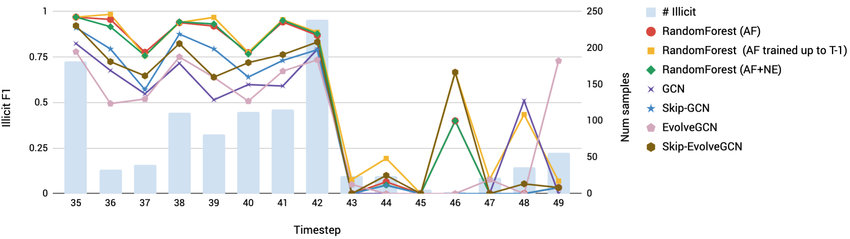
\includegraphics[width=\textwidth]{images/elliptic-fraud-f1.png}
    \caption{F1 evolution facing a crash in the elliptic dataset. At time t=43, the sudden disappearance of a Dark Market has a notable adverse impact on the performance of all models in subsequent periods.\cite{bellei_elliptic_2019}}
    \label{fig:elliptic-fraud-f1}
\end{figure}

\textbf{Classical machine learning techniques} like support vector machines (SVMs), XGBoost, or random forests can also provide some form of interpretability. These models are generally easier to understand and provide insights into the importance of different graph features. Including graph features enrichment can even improve the accuracy of classical models to a level comparable to GNNs\cite{rao_modelling_2022}! Graph feature enrichment involves extracting meaningful features (e.g., neighborhood information) from the graph structure to enhance the predictive power of the model.

\begin{figure}
    \centering 
    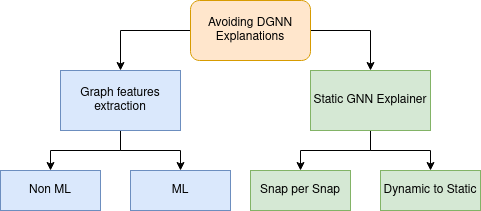
\includegraphics[width=0.75\textwidth]{images/avoiding-dgnn-diagram.png}
    \caption{Avoiding dynamic GNN explainers}
    \label{fig:avoiding-dgnn-diagram}
\end{figure}

A different, counter-intuitive alternative to using dynamic GNN explainers is modifying static GNN explainers. There are two ways to adapt them:

\textbf{Snapshot-per-snapshot explanation} involves providing explanations for each snapshot of the dynamic graph individually, without considering time evolution. By focusing on each snapshot independently, this method is simple and provides explanations that are specific to the features and relationships within that particular snapshot. This has one main limitation: \textit{losing temporal context}. Dynamic graphs often have time-dependent patterns and relationships that can influence the behavior of the network, leading to incomplete or misleading explanations. Despite this, we argue that static GNN explainers may be a good fit for a temporal GNN in many scenarios.

\textbf{Transforming dynamic graphs into a static graph} involves augmenting the dynamic graph by adding temporal edges, effectively transforming it into a static graph\cite{kim_temporal_2022}. By adding temporal edges, the transformed static graph retains the temporal relationships between different snapshots. This allows for the utilization of traditional static GNN explainers while still considering the time evolution of graphs. These explanations can then reflect the influence of temporal dependencies on the GNN's behavior. However, transforming a dynamic graph into a static graph by adding temporal edges introduces additional complexity. Pruning the graph and modifying the explainer to each specialized static graph might be necessary. We found no papers on this topic, but we expect it to be a topic in future research.

The choice between each of the two static GNN explainer methods depends on the target problem, importance of temporal context, and trade-off between simplicity and capturing temporal dynamics.

\subsection{Dynamic GNN explanation}
Table \ref{table-3-full} was already introduced in section 2.4, but we include further details on the papers here. These papers try to combine the best of both machine learning accuracy and and a human understandable model-decision process.
\begin{itemize}
    \item STpGCN\cite{ye_explainable_2023} captures the spatial-temporal graph representation of brain activities by incorporating multi-scale temporal dependency via graph structures. In addition, the paper introduces a sensitivity analysis method called BrainNetX, which automatically annotates task-related brain regions from a brain-network standpoint, enhancing the explainability of decoded results while validating the hierarchical structure of STpGCN.
    \item TGNNExplainer\cite{he_explainer_2022} framework consists of two modules: the first module explains each time step prediction independently using a probabilistic graphical model, and the second module discovers the dominant interesting explanations in a time period.
    \item DGExplainer\cite{xie_explaining_2022} redistributes the output activation scores of a dynamic GNN to the neurons in its previous layer, creating input neuron relevance scores. The input relevance explains the model decision.
    \item XHGP\cite{limeros_towards_2022} utilizes GNNExplainer, attention, and counterfactual reasoning to improve the prediction explanations. The model is being developed for autonomous vehicles, with its graph and challenges unique to that field.
    \item GCN-SE\cite{fan_gcn-se_2021} uses squeeze and excitation to find snapshot attention weights, illustrating the predictive power of attention interpretability.
    \item RNN-GCN\cite{yao_interpretable_2021} weights each edge based on its longevity. A decay rate is used to lower edge importance as time goes on. An optimal decay is calculated for each cluster and is interpreted as importance of historical connection information.
    \item FraudMemory\cite{yang_fraudmemory_2019} computes three fraud scores: sequential, group, and individual fraud score. FraudMemory merges them to make a final prediction. The three scores can each be viewed as a  potential source of anomalies. The subscores also contribute to both model decisions and interpretation of fraudulent behavior.
\end{itemize}

Certain dynamic graph neural networks (GNNs) employ attention mechanisms, decay rates, or sub-scores to enhance interpretability. While interpretability is advantageous due to its inherent transparency without requiring a post-hoc explainer, it has limitations and cannot, for instance, calculate feature importance\cite{yao_interpretable_2021}. Therefore, interpretability and explainability should be regarded as complementary aspects rather than substitutes. If a higher level of transparency and comprehension of the model is desired, dynamic explainers can be employed on top of an interpretable GNN.

\clearpage
\begin{figure}
    \centering
    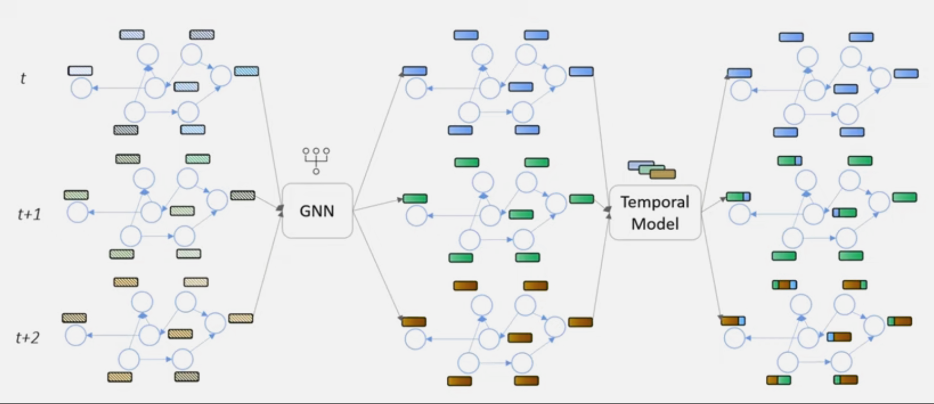
\includegraphics[width=\textwidth]{images/tgn-embedding-white.png}
    \caption{TGN and Spacio-temporal embeddings \cite{deepfindr_friendly_2021}. The raw snapshots on the left side are subjected to processing by a static GNN. In the middle, the snapshots incorporate spatial information as a result of message passing and aggregation. On the right side, the static spatial information of each node is combined over time to create a spatio-temporal embedding. In other words, previous embeddings are used as node history.}
    \label{fig:tgn-embedding}
\end{figure}

Using only a slightly-modified GNN explainer in specific contexts can produce striking results:
\begin{enumerate}
    \item Consider that gradient, surrogate, perturbation and decomposition methods can be used for dynamic GNNs in the same way they would normally used for static graphs. This is possible because node embeddings contain \textit{all} necessary temporal information. Apply one of these methods to a dynamic graph dataset.
    \item Continue by attaching an GNN explainer to this model that processes each snapshot individually.
    \item Aggregate the node embeddings, and collect the result.
\end{enumerate}

This is the process illustrated in figure \ref{fig:tgn-embedding}. All the temporal, spatial and feature information is being gathered on the embeddings in the bottom-right corner of the figure. A static explainer is able to perfectly explain the importance of each part of these embeddings; this implies that dynamic explainers are not needed for models that combine all information into one embedding. This is significant because this is practice for graphs where nodes don't appear or disappear often. The need for dynamic specific explainability is therefore mostly limited to dynamic graphs that strongly vary over time.

% ---- Discussion ----
\section{Discussion \& Critical Reflection}
\subsection{Experimental Method Proposal}
To encourage further research in this direction, we provide a sample reproducible explainability experiment. This includes dataset selection, graph formation and pre-processing, anomaly detection selection, and a compatible explainer. We provide both assumptions and examples within the context of fraud detection, with recommendations for results validation and ethical considerations.

\subsubsection{Dataset Selection and Pre-processing}
Both synthetic and real datasets are advantageous when creating or evaluating explainability models. Results generated from synthetic injected datasets can benefit from ground truth and supervision, while real data remains necessary to generalize models for real-world scenarios and train models on hidden complexities unaccounted for in generated data. The following fraud examples fulfill these requirements and are time-varying:

\begin{itemize}
    \item \textit{Elliptic dataset}\cite{weber_anti-money_2019}: a real cryptocurrency transaction dataset published by Weber, Domeniconi et al. and maintained by Elliptic.co.
    \item  \textit{BankSim dataset}\cite{lopez-rojas_banksim_2014}: a synthetic bank transaction dataset created by Dr. Lopez-Rojas.
    \item \textit{PaySim dataset}\cite{lopez-rojas_applying_2016}: a synthetic merchant transaction dataset created by Dr. Lopez-Rojas.
    \item \textit{Ebay dataset}\cite{rao_xfraud_2021}: a real customer transaction dataset curated by xFraud and licensed from Ebay Inc.
\end{itemize}

The following steps will utilize elliptic dataset due to its real data, generous licensing, and temporal graph structure. Elliptic transaction dataset is a collection of Bitcoin transactions that have been mapped and labeled specifically for financial network analysis and forensics. Each graph snapshot contains information about individual Bitcoin transactions, including the transaction ID, timestamp, input and output addresses, and the amount of Bitcoin transferred. Of the 203,769 nodes and 234,355 edges, only 23\% are labeled as either legitimate or illicit based on known fraudulent involvement\cite{weber_anti-money_2019}. Unfortunately, this means that the underlying model we choose to explain can't be monitored for performance via its true positive rate or true negative rate (sensitivity and specificity).

The common graph formation approach for this dataset is to represent nodes as transactions, with edges representing the flow of Bitcoin between transactions:

\clearpage
\begin{figure}
    \centering 
    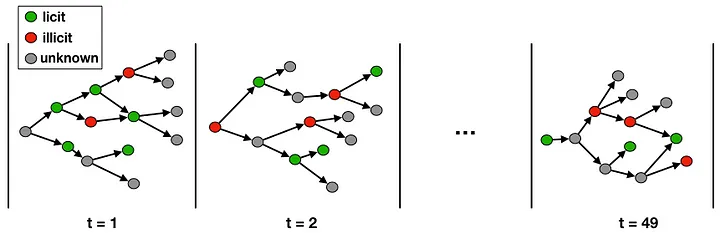
\includegraphics[width=\textwidth]{images/elliptic-sub-snap.png}
    \caption{Visualizatoin of elliptic subgraph structure over time \cite{bellei_elliptic_2019}. The Bitcoin blockchain is a directed acyclic graph (DAG). The Elliptic Data Set contains 49 connected components, from the earliest one at time step t = 1 to the later one at time step t = 49.}
    \label{fig:elliptic-sub-graphs}
\end{figure}

Transaction graphs that encode information in this format can be more difficult to analyze, as each node appears only once within a single time interval. This means that there is no node evolution between time intervals, making historical association difficult. Even though each time interval snapshot can be treated as a temporal graph, prior snapshots need to enhance classification using some other pattern or dimension because nodes will never reappear. This has interesting implications, as it suggests temporal models and explainers trained on traffic or brain prediction in other domains aren't suitable for transaction data in this arrangement. Based on our observation, most methods using node embeddings depend on node propagation history as an input and are also unsuitable. In fact, none of the models presented in Table \ref{table-3-full} are useful here due to the nature of the elliptic graphs. This example illustrates the importance of graph structure on model choice. EvolveGCN \ref{fig:EvolveGCN} shows how models can still effectively capture this temporal information using alternatives like LSTM or GRU. Trying to avoid this node embedding problem by mapping Bitcoin senders and receivers to nodes would create its own set of constraints: all temporal information would need to be re-encoded as edge features, and less developed edge embedding solutions would need to be used.

\subsubsection{Anomaly Detection Model Selection}
When selecting a detection model, it is important to consider compatibility, performance, and support for established frameworks. Since Elliptic dataset encodes temporal information via time-step, we need to focus on temporal graph analysis models.

Some preliminary analyses process the formed elliptic graphs through the use of GCNs\cite{karthika_gcn_2021}\cite{yang_transfer_2020} and autoencoder\cite{soto_fraud_2021}, though an existing published implementation exists via EvolveGCN\cite{pareja_evolvegcn_2019}.

DyHGN\cite{rao_modelling_2022} is another possiblility, as it was designed to deal with dynamic heterogeneous fraudulent transactional graphs. DyHGN is a dynamic extension of xFraud\cite{rao_xfraud_2021}, but unlike xFraud DyHGN uses Shapley Values instead of a GNNexplainer to explain graph-features via ab enriched XGBoost technique. This way, DyHGN avoids the complexity of explaining a dynamic heterogeneous network while benefiting from increased accuracy.

EvolveGCN\cite{pareja_evolvegcn_2019} is a RNN-GCN, using an RNN (via LSTM or GRU) to evolve its GCN's weights. Unlike the more common GCN-RNN proposed by \cite{narayan_learning_2018} and \cite{xie_explaining_2022} that suffers from cold starts, an RNN-GCN is able to predict fully dynamic graphs like Elliptic data. The main advantage of this technique is that it allows static explainers to be used. Amara et al.\cite{amara_graphframex_2022} mentions the effectiveness of perturbation technique for fraud explanation, and a GNNExplainer or modified GNNExplainer as proposed by \cite{rao_xfraud_2021} could be adapted to show important node/edge features that influenced specific instance classifications.

When selecting a model for graph analysis, code availability and support for established frameworks can be just as important as  for contributing reproducible, novel outcomes. Plan your technical implementation of the model around the intention to integrate the model, explainer, and dataset into a project like PyG\cite{pyg_team_pyg_nodate} or \cite{liu_pygod-teampygod_2023}. A meta framework like \cite{dive_lab_dig_nodate} may also be helpful in standardizing your data preparation and explainer wrapper with other implementations being developed.

\subsubsection{Explainers Selection}
The output of your anomaly detection model will be in the form of vectors containing anomalous embeddings. This is one of two components taken as an input into explainers. The other component will be some form of interfacing parameter that introspects EvolveGCN's black box process. We recommend picking a compatible temporal explainer to adapt based on the following criteria, in order of importance:

\begin{itemize}
    \item Actively developed with code available
    \item Merged into existing frameworks
    \item Published or used in order scenarios
    \item Known authors
\end{itemize}

We would advise against implementing the original EvolveGCN source; the temporal snapshot version of Elliptic has been recently integrated into PyG, and it would be both more novel and more reproducible for others to implement your model and explainer in PyG.

\subsubsection{Evaluation and Validation Metrics}
Evaluation and validation help quantify and verify the results of their machine learning models and explainers. If ground truth is available, check the underlying model's proportion of anomalies to total observations; if graphs are highly sparse, there is a higher proportion of false positives\cite{zhang_trustworthy_2022}. Fidelity scores can be used to measure precision via recall or F1 scores, as appropriate. Perturbation can be used after-the-fact to perform a sensitivity analysis to check which inputs most heavily affect explainer attributions. This could also be a potential source of bias.

Additional cross-validation with or without bootstrapping can be used to identify potential under- or over-fitting. This is accomplished by partitioning an existing dataset into training and validation sets, iteratively testing random subsets to evaluate performance on new data. Cross-validating with bootstrapping would require resampling the dataset and generating new subsets to evaluate variability and stability via distribution\cite{kauermann_statistical_2021}.

\subsection{Future Directions}
Further development of interpretability in dynamic graphs: Interpretability is highly valuable as it reduces the need for a secondary explanation model. The ongoing effort lies in developing accurate machine learning models that are inherently interpretable. However, there is still progress to be made in the field of time-specific interpretability, in areas like snap attention which are still in early stages of development.

Merging parallel work on GCN data loaders, explainable models, and frameworks: Merge orphan anomaly detection models and associated explainers into a parent framework like PyG, PyGoD, or Dive into Graphs to create a more reproducible research environment for the community.

Systems for streaming heterogenous graph data, live timestep-aware explainers: Contribute directly to the PyG team in an effort to adapt and implement live temporal or dynamic graph streaming.

Cost-aware models: Finding the optimal balance between true positives (TP) and false positives (FP) presents a significant challenge. However, by assigning costs to TP and FP, it becomes feasible to identify the most financially advantageous model for companies.

Performing a systematic analysis of bank costs associated with false positives (overly sensitive) and false negatives (camouflaging) due to the implementation of a cost-aware detection model is crucial in financial systems. Surprisingly, there are only a limited number of papers that specifically focus on cost considerations for the bank or companies in this context. Therefore, developing a cost aware detection model is a potential avenue for future research.

Model-based explanation: Instance-based explanations have seen greater development compared to model-based explanations. This is primarily due to the challenge of comprehending a large and complex set of rules that arise when attempting to explain the entire model's decision for all nodes. However, in cases where the graph is small or when anomalies exhibit redundant patterns, model-based explanations can be beneficial.

For dynamic graphs, we propose exploring snap-based explanations, which can be particularly valuable when encountering frequently processing similar fraud data. Additionally, snapshot graphs tend to be smaller than static graphs since more snapshots need to be stored. This presents a potential application for model/snapshot-based explainers.

% ---- Conclusion ----
\section{Conclusion}
The scope of this study encompassed a comprehensive overview of dynamic anomaly detection and explainability methods, noting their importance in fraud-specific applications. By addressing existing potential challenges and providing future directions for explainability development, it attempts to encourage future growth in this research space.

Reflecting on novel developments in this field allowed for the proposal of a holistic experimental method that covers essential considerations from data selection and pre-processing through to explainer validation. We make special emphasis on the potential of modified static explainers for temporal models. Our work ultimately aims to serve as both a guide towards practical experimental application, and a time-saving source of up-to-date information. It seeks to play at least a small part in paving the way for more interpretable, quantifiable machine learning decisions that can be applied across specialties.
\clearpage

% ---- Bibliography ----
\bibliographystyle{splncs04}
\bibliography{bibliography-zotero} \label{references}

% ---- Appendices ----
\appendix
\section*{Appendix}
\addcontentsline{toc}{section}{Appendix}
\section{Trend Data for Explainability papers}
\begin{figure}[h]
    \centering
    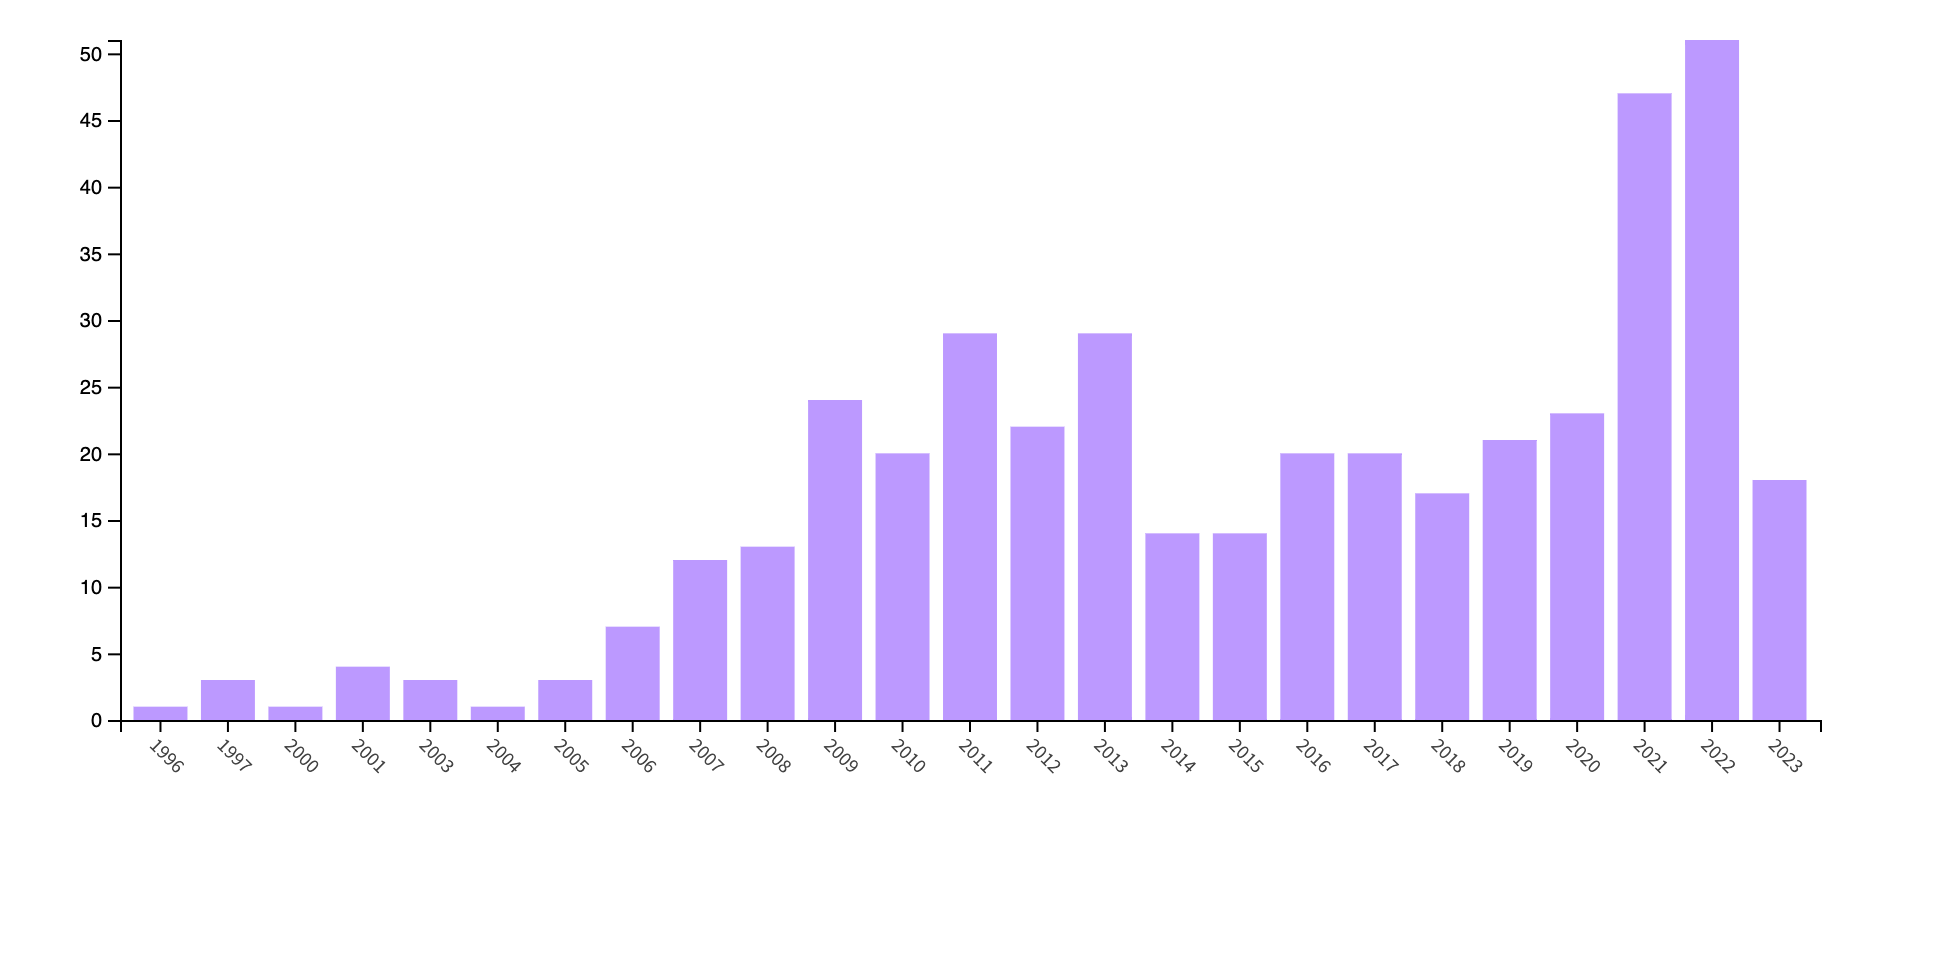
\includegraphics[width=.75\textwidth]{images/publications-keywords.jpg}
    \caption{
    Number of publications published per year with keywords (inclusive OR): explainable, explainability, explainer, interpretable, interpretability. Data and graphic included herein is derived from Clarivate Web of Science. © Copyright Clarivate 2023. All rights reserved.}
    \label{fig:publications-keywords}
\end{figure}

\section{EvolveGCN Temporal Layer Weighting}
\begin{figure}[h]
    \centering
    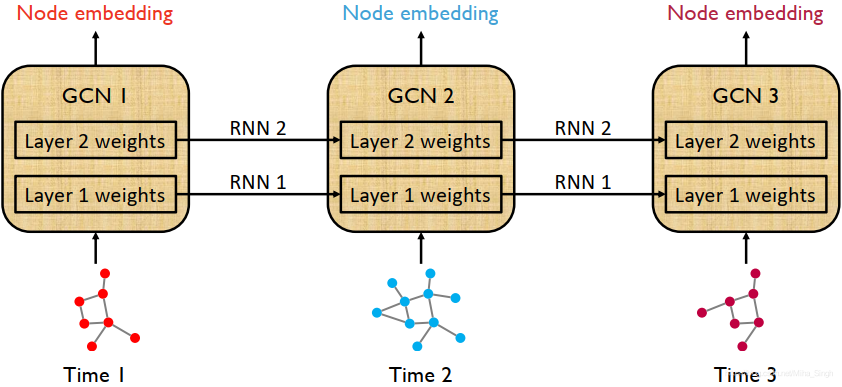
\includegraphics[width=.75\textwidth]{images/evolve-gcn.png}
    \caption{Layer parameters are evolved over time via RNN\cite{pareja_evolvegcn_2019}. Each snapshot has its own GCN. Temporal information is used to upgrade the weights matrix.}
    \label{fig:EvolveGCN}
\end{figure}

\section{Table 3. GNN Prediction and Explanation in Dynamic Graphs}
\begin{sidewaystable}
    \centering
    \begin{tabular}{|l|l|l|l|l|l|l|l|l|}
        \hline
        Paper & Year & Technique & Technique class & Explanation & Black Box & Task* & Graph & Application \\ \hline
        Ye et al.\cite{ye_explainable_2023} & 2023 & BrainNetX & Gradient(SA) & Node & STpGCN & NC & Temporal & brain \\
        He et al.\cite{he_explainer_2022} & 2022 & TGNNExplainer & Surrogate(PGM) & Subgraph & TGNN & NOP & Temporal & traffic \\
        Limeros et al.\cite{limeros_towards_2022} & 2022 & XHGP & Perturbation(counterfactual) & Interaction & GAT-GRU & MP & Temporal & autonomous cars \\
        Xie et al.\cite{xie_explaining_2022} & 2022 & DGExplainer & Decomposition(LRP) & Features & GCN-GRU & NR & Dynamic & traffic \\
        Fan et al.\cite{fan_gcn-se_2021} & 2022 & Interpretability & Attention & Snapshot & GCN-SE & NC & Dynamic & bibliography \\
        Yao et al.\cite{yao_interpretable_2021} & 2021 & Interpretability & Decay rate & Edge & RNN-GCN & NC & Edge Dynamic& bibliography \\
        Yang et al.\cite{yang_fraudmemory_2019} & 2019 & Interpretability & Sub Scores & Time & FraudMemory & NC & Edge Dynamic & Fraud \\
        \hline
    \end{tabular}
    *NC= node classification, NOP= node output prediction, NR=node regression, MP=motion prediction
    \label{table-3-full}
\end{sidewaystable}

\clearpage

% ---- List of figures ----
\listoffigures

% ---- List of tables ----
\listoftables

\end{document}